\item O volante $A$ de \SI{15}{\kilogram} tem um raio de giração em relação a seu centro de \SI{100}{\milli\meter}. O disco $B$ tem uma massa de \SI{25}{\kilogram} e está acoplado ao volante através de uma correia que não desliza em suas superfícies de contato. Se um motor fornece ao volante um torque no sentido anti-horário $M=(75t)\,\SI{}{\newton\cdot\meter}$, onde $t$ é dado em segundos, determine o tempo necessário para o disco alcançar uma velocidade angular de \SI{60}{\radian/\second} partindo do repouso.

\import{../answers}{answer-7}

\begin{flushright}
	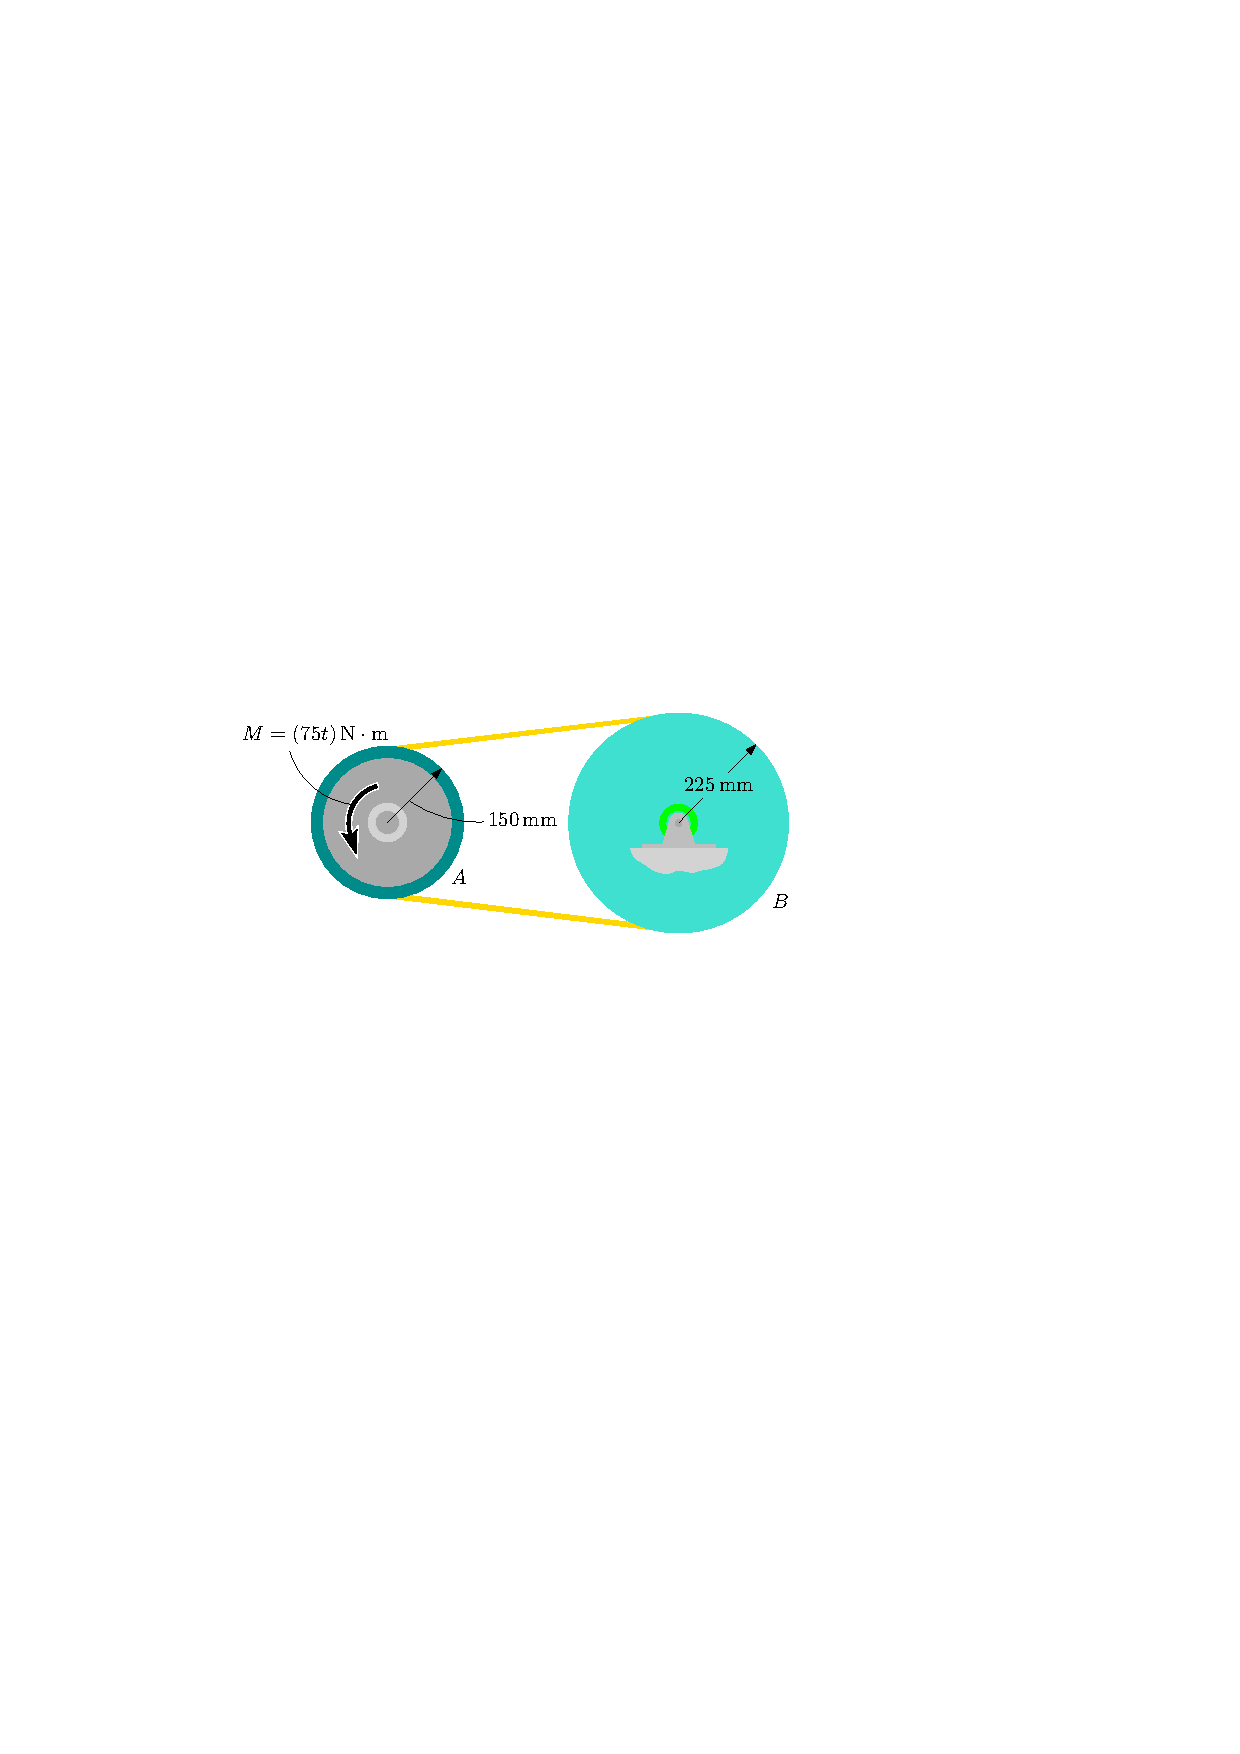
\includegraphics[scale=1.1]{../../images/draw_4}
\end{flushright}
